\section{Unimodality constraint using Monotonicity}
The latent derivative function $m$ in equation \ref{linkfunc} can be modeled as an input dependant function which can be used to enforce shape constraints. The unimodality information can be modelled by a using parameteric monotonic function to represent the derivative information $m$. The primary role of the monotonic derivative function model would be to learn the mode of the data accurately, where the sign of the derivative would flip. 

We experimented with three different models for the latent derivative function:
\begin{enumerate}
	\item Linear model of the form $m(x)=ax+b$
	\item A zero mean Gaussian process of the form $m(x)=GP(0,k_m(x,x))$
	\item A linear mean Gaussian process $m(x)=GP(ax+b,k_m(x,x))$ 
\end{enumerate}

\begin{figure}[h]
  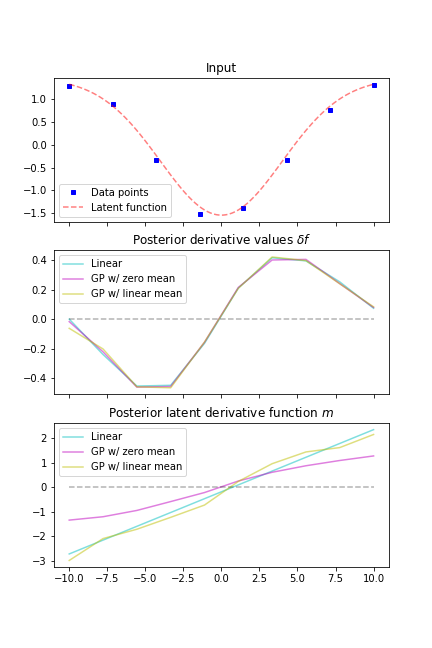
\includegraphics[scale=0.7]{monotonicity.png}
  \centering
  \caption{Example of model}
  \label{fig:unimodality_exp}
\end{figure}

Figure \ref{fig:unimodality_exp} shows how the unimodality constraint develops under the given model.



